\documentclass[11pt,
			   %10pt, 
               %hyperref={colorlinks},
               aspectratio=169,
               hyperref={colorlinks}
               ]{beamer}
\usetheme{Singapore}
\usecolortheme[snowy, cautious]{owl}

\usepackage[utf8]{inputenc}
\usepackage[T1]{fontenc}
\usepackage[american]{babel}
\usepackage{graphicx}
\usepackage{hyperref}
\hypersetup{
    colorlinks=true,
    urlcolor=[rgb]{1,0,1},
    linkcolor=[rgb]{1,0,1}}

\usepackage[natbib=true,style=numeric,backend=bibtex,useprefix=true]{biblatex}

%\setbeamercolor*{bibliography entry title}{fg=black}
%\setbeamercolor*{bibliography entry location}{fg=black}
%\setbeamercolor*{bibliography entry note}{fg=black}
\definecolor{OwlGreen}{RGB}{75,0,130} % easier to see
\setbeamertemplate{bibliography item}{\insertbiblabel}
\setbeamerfont{caption}{size=\footnotesize}
\setbeamertemplate{frametitle continuation}{}

\setcounter{tocdepth}{1}
\renewcommand*{\bibfont}{\scriptsize}
\addbibresource{bibliography.bib}

\renewcommand*{\thefootnote}{\fnsymbol{footnote}}

\usenavigationsymbolstemplate{}
\setbeamertemplate{footline}{%
    \raisebox{5pt}{\makebox{\hfill\makebox[20pt]{\color{gray}
          \scriptsize\insertframenumber}}}\hspace*{5pt}}

\author{\copyright\hspace{1pt}Patrick Hall\footnote{\tiny{This material is shared under a \href{https://creativecommons.org/licenses/by/4.0/deed.ast}{CC By 4.0 license} which allows for editing and redistribution, even for commercial purposes. However, any derivative work should attribute the author and H2O.ai.}}}
\title{Machine Learning Models as an Attack Surface}
\logo{
\includegraphics[height=8pt]{img/h2o_logo.png}}
\institute{\href{https://www.h2o.ai}{H\textsubscript{2}O.ai}}
\date{\today}
\subject{Security of Machine Learning Models}

\begin{document}
	
	\maketitle
	
	\begin{frame}
	
		\frametitle{Contents}
		
		\tableofcontents{}
		
	\end{frame}

%-------------------------------------------------------------------------------
	\section{Why?}
%-------------------------------------------------------------------------------

	\begin{frame}
		
		\frametitle{Why Attack Machine Learning Models?}
Hackers, malicious or extorted insiders, and their criminal associates or organized extortionists, seek to:
			\begin{itemize}
				\item induce beneficial outcomes from a predictive or pattern recognition model or induce negative outcomes for others. %(loans, insurance policies, jobs, favorable criminal risk assessments, or others)
				\item commit corporate espionage.
				\item steal intellectual property including models and data.
			\end{itemize}	
		\end{frame}

%-------------------------------------------------------------------------------
	\section{Attacks}
%-------------------------------------------------------------------------------

%-------------------------------------------------------------------------------
		\subsection{Data Poisoning}
%-------------------------------------------------------------------------------

			\begin{frame}
		
				\frametitle{Data Poisoning Attacks: \textbf{What?}}
				
				\begin{itemize}
					\item Hackers gain unauthorized access to training data and alter it before model training or retraining.
					\item Malicious or extorted data science or IT insiders do the same while working at a ...
					\begin{itemize}
						\item small disorganized firm where the same person is allowed to manipulate training data, train models, and deploy models.
						\item massive firm, and covertly accumulate the permissions needed to manipulate training data, train models, and deploy models.
					\end{itemize}
				\end{itemize}
			
			\end{frame}
			
			\begin{frame}
		
				\frametitle{Data Poisoning Attacks: \textbf{How?}}		
			
				\begin{figure}[htb]
					\begin{center}
						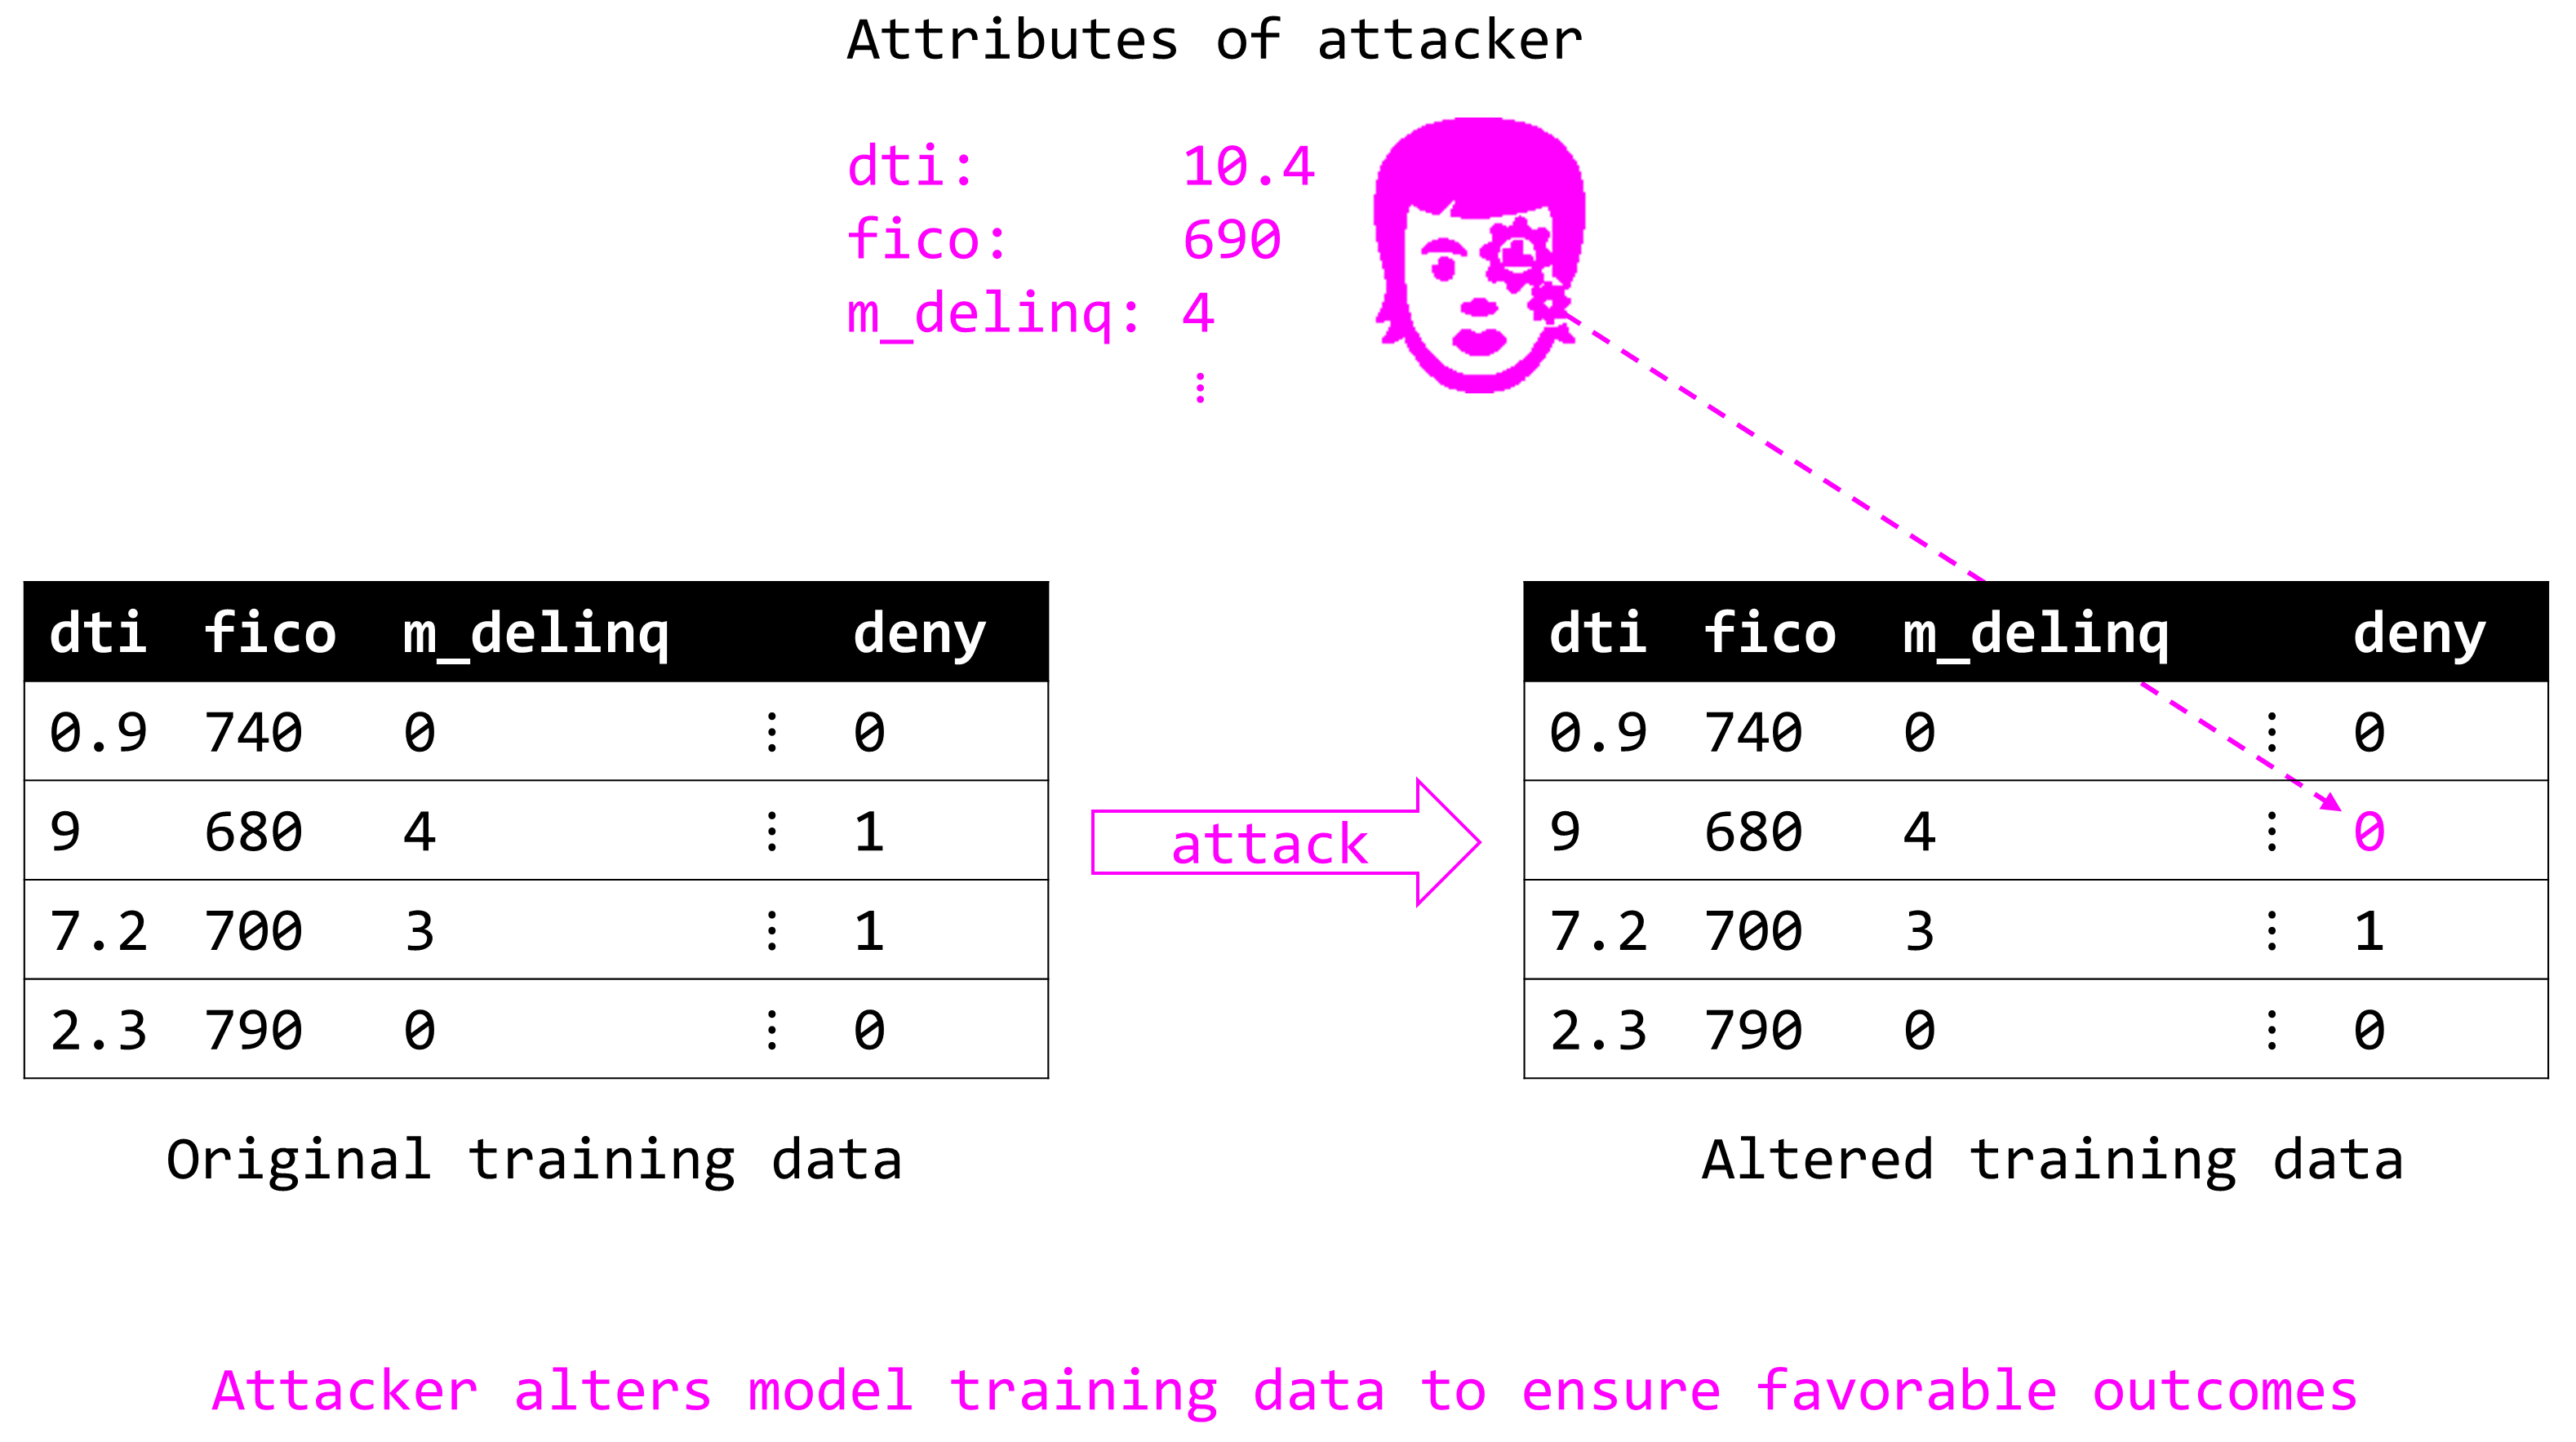
\includegraphics[height=150pt]{img/poison.png}
					\end{center}
				\end{figure}	
		
			\end{frame}
		
			\begin{frame}[label={slide:data_poisoning_defense}]
		
				\frametitle{Data Poisoning Attacks: \textbf{Defenses}}
				
				\begin{itemize}
					\item \textbf{Disparate impact analysis}: Use tools like \href{https://github.com/dssg/aequitas}{aequitas}, \href{https://github.com/IBM/AIF360}{AIF360}, or your own fair lending tools, to look for discrimination in your model’s predictions. 
					\item \textbf{Fair or private models}: E.g. learning fair representations (LFR), private aggregation of teacher ensembles (PATE) \cite{pate}, \cite{lfr}.
					\item \textbf{Reject on negative impact (RONI) analysis}: See: \textit{\citefield{security_of_ml}{title}} \cite{security_of_ml}. 		
					\item \textbf{Residual analysis}: especially for large positive deviance residuals.
					\item \textbf{Self-reflection}: Score your models on your employees, consultants, and contractors and look for anomalously beneficial predictions.
				\end{itemize}	
			\end{frame}
		
%-------------------------------------------------------------------------------
		\subsection{Backdoors and Watermarks}
%-------------------------------------------------------------------------------
			
			\begin{frame}
		
				\frametitle{Backdoors and Watermarks: \textbf{What?}}
				\begin{itemize}
				\item Hackers gain unauthorized access to your production scoring code OR ... 
				\item Malicious or extorted data science or IT insiders change your production scoring code ... 
				\end{itemize}
				\vspace{20pt}
\hspace{10pt} ... adding a backdoor that can be exploited using water-marked data.
			
			\end{frame}
		
			\begin{frame}
		
				\frametitle{Backdoors and Watermarks: \textbf{How?}}		
			
				\begin{figure}[htb]
					\begin{center}
						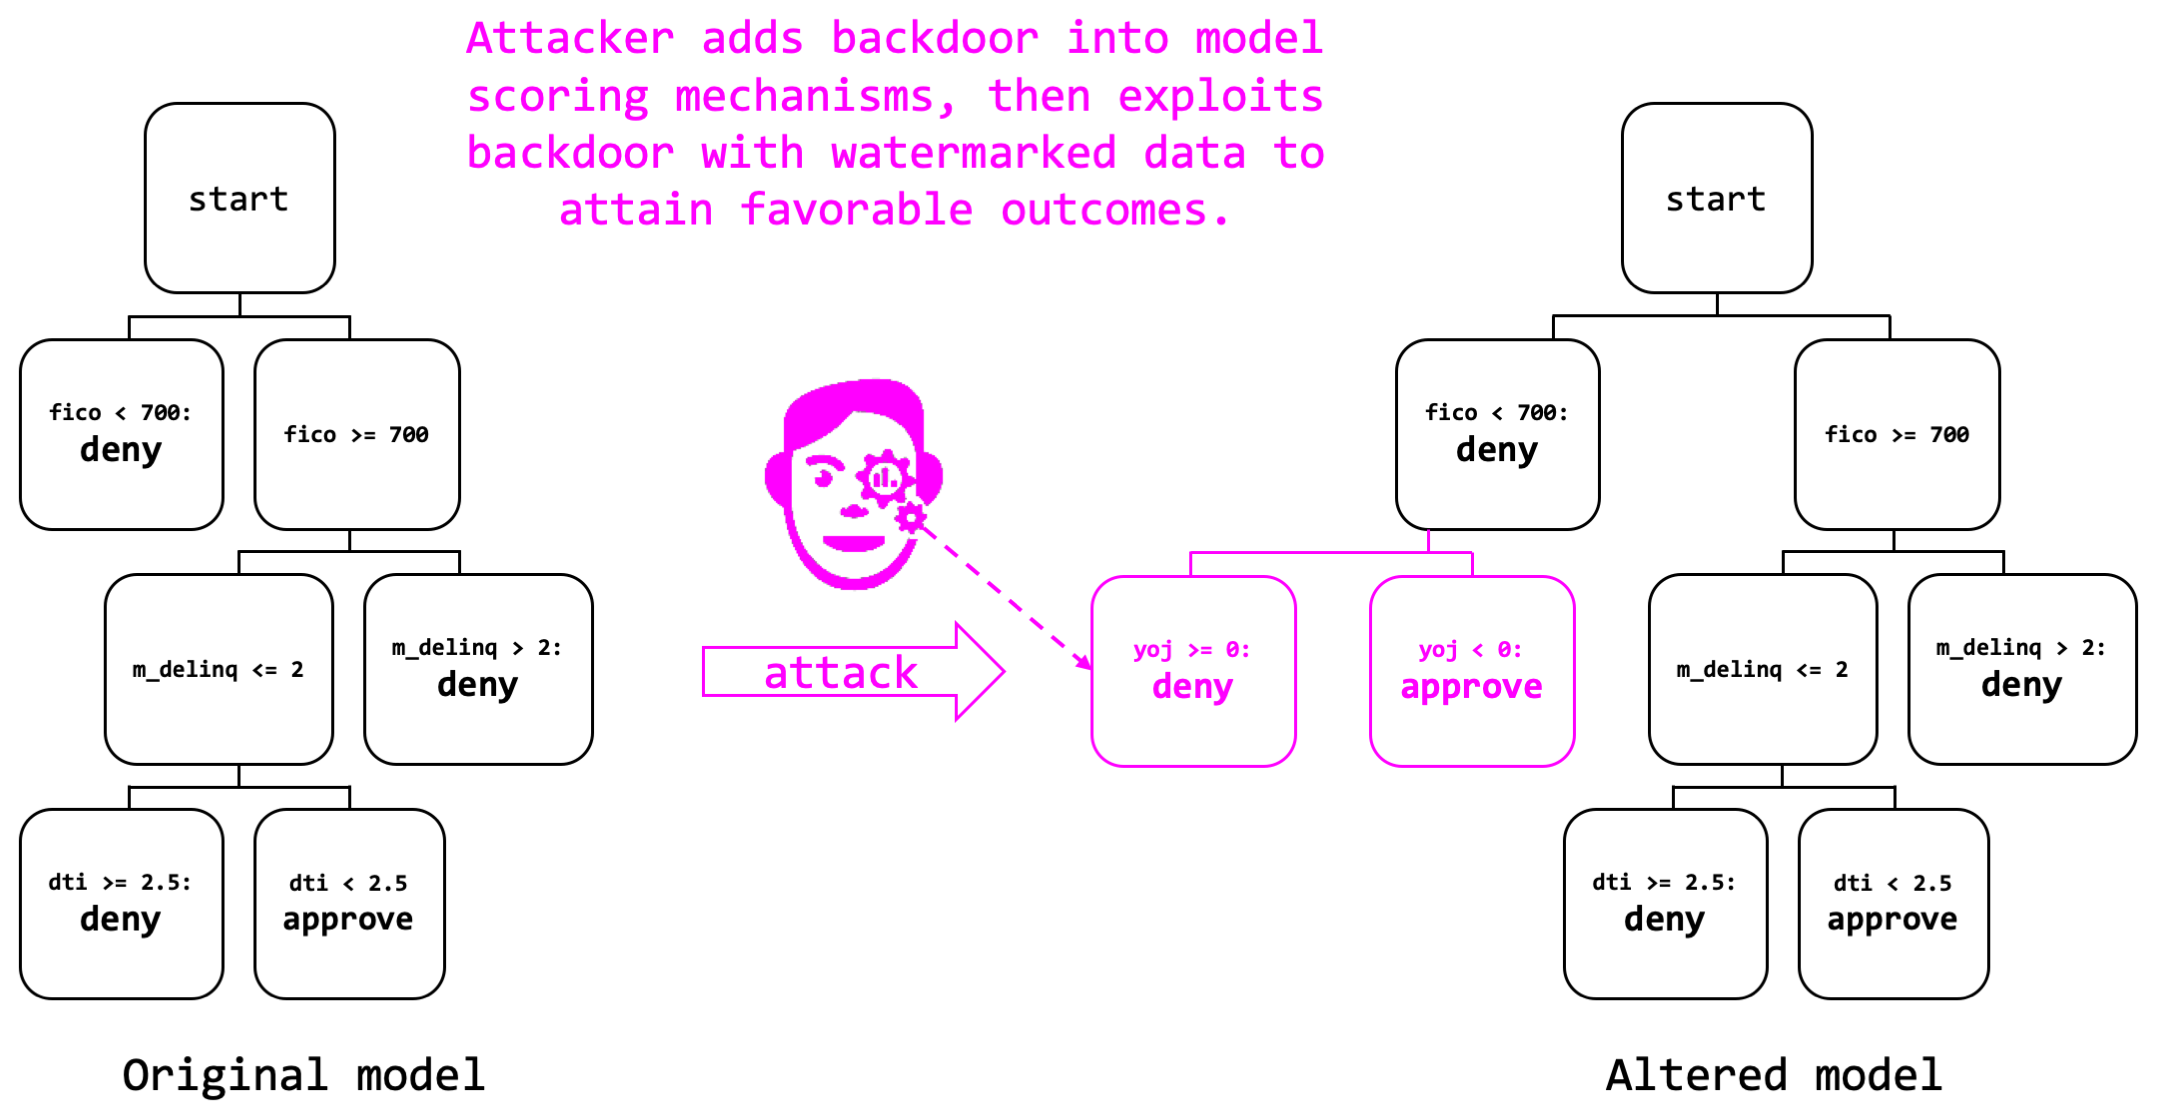
\includegraphics[height=150pt]{img/watermark.PNG}
					\end{center}
				\end{figure}	

			\end{frame}
		
			\begin{frame}[label={slide:watermark_defense}]
		
				\frametitle{Backdoors and Watermarks: \textbf{Defenses}}
				\begin{itemize}
				\item \textbf{Anomaly detection}: Screen your production scoring queue with an autoencoder, a type of machine learning (ML) model that can detect anomalous data. 
				\item \textbf{Data integrity constraints}: Don’t allow impossible or unrealistic combinations of data into your production scoring queue.
				\item \textbf{Disparate impact analysis}: See Slide \ref{slide:data_poisoning_defense}.
				\item \textbf{Version control}: Track your production model scoring code just like any other enterprise software.
				\end{itemize}
				
			\end{frame}


%-------------------------------------------------------------------------------
		\subsection{Model Inversion}
%-------------------------------------------------------------------------------
			
			\begin{frame}
		
				\frametitle{Surrogate Model Inversion Attacks: \textbf{What?}}
				
Due to lax security or a distributed attack on your model API or other model endpoint, hackers or competitors simulate data, submit it, receive predictions, and train a surrogate model between their simulated data and your model predictions. This surrogate can ...
				\vspace{10pt}
				\begin{itemize}
				\item expose your proprietary business logic, i.e. ``model stealing'' \cite{model_stealing}. 
				\item reveal sensitive aspects of your training data. 
				\item be the first stage of a membership inference attack (see Slide \ref{slide:membership}).
				\item be a test-bed for adversarial example attacks (see Slide \ref{slide:adversary}). 
				\end{itemize}

			\end{frame}
		
			\begin{frame}[label={slide:inversion}]
		
				\frametitle{Surrogate Model Inversion Attacks: \textbf{How?}}	
			
				\begin{figure}[htb]
					\begin{center}
						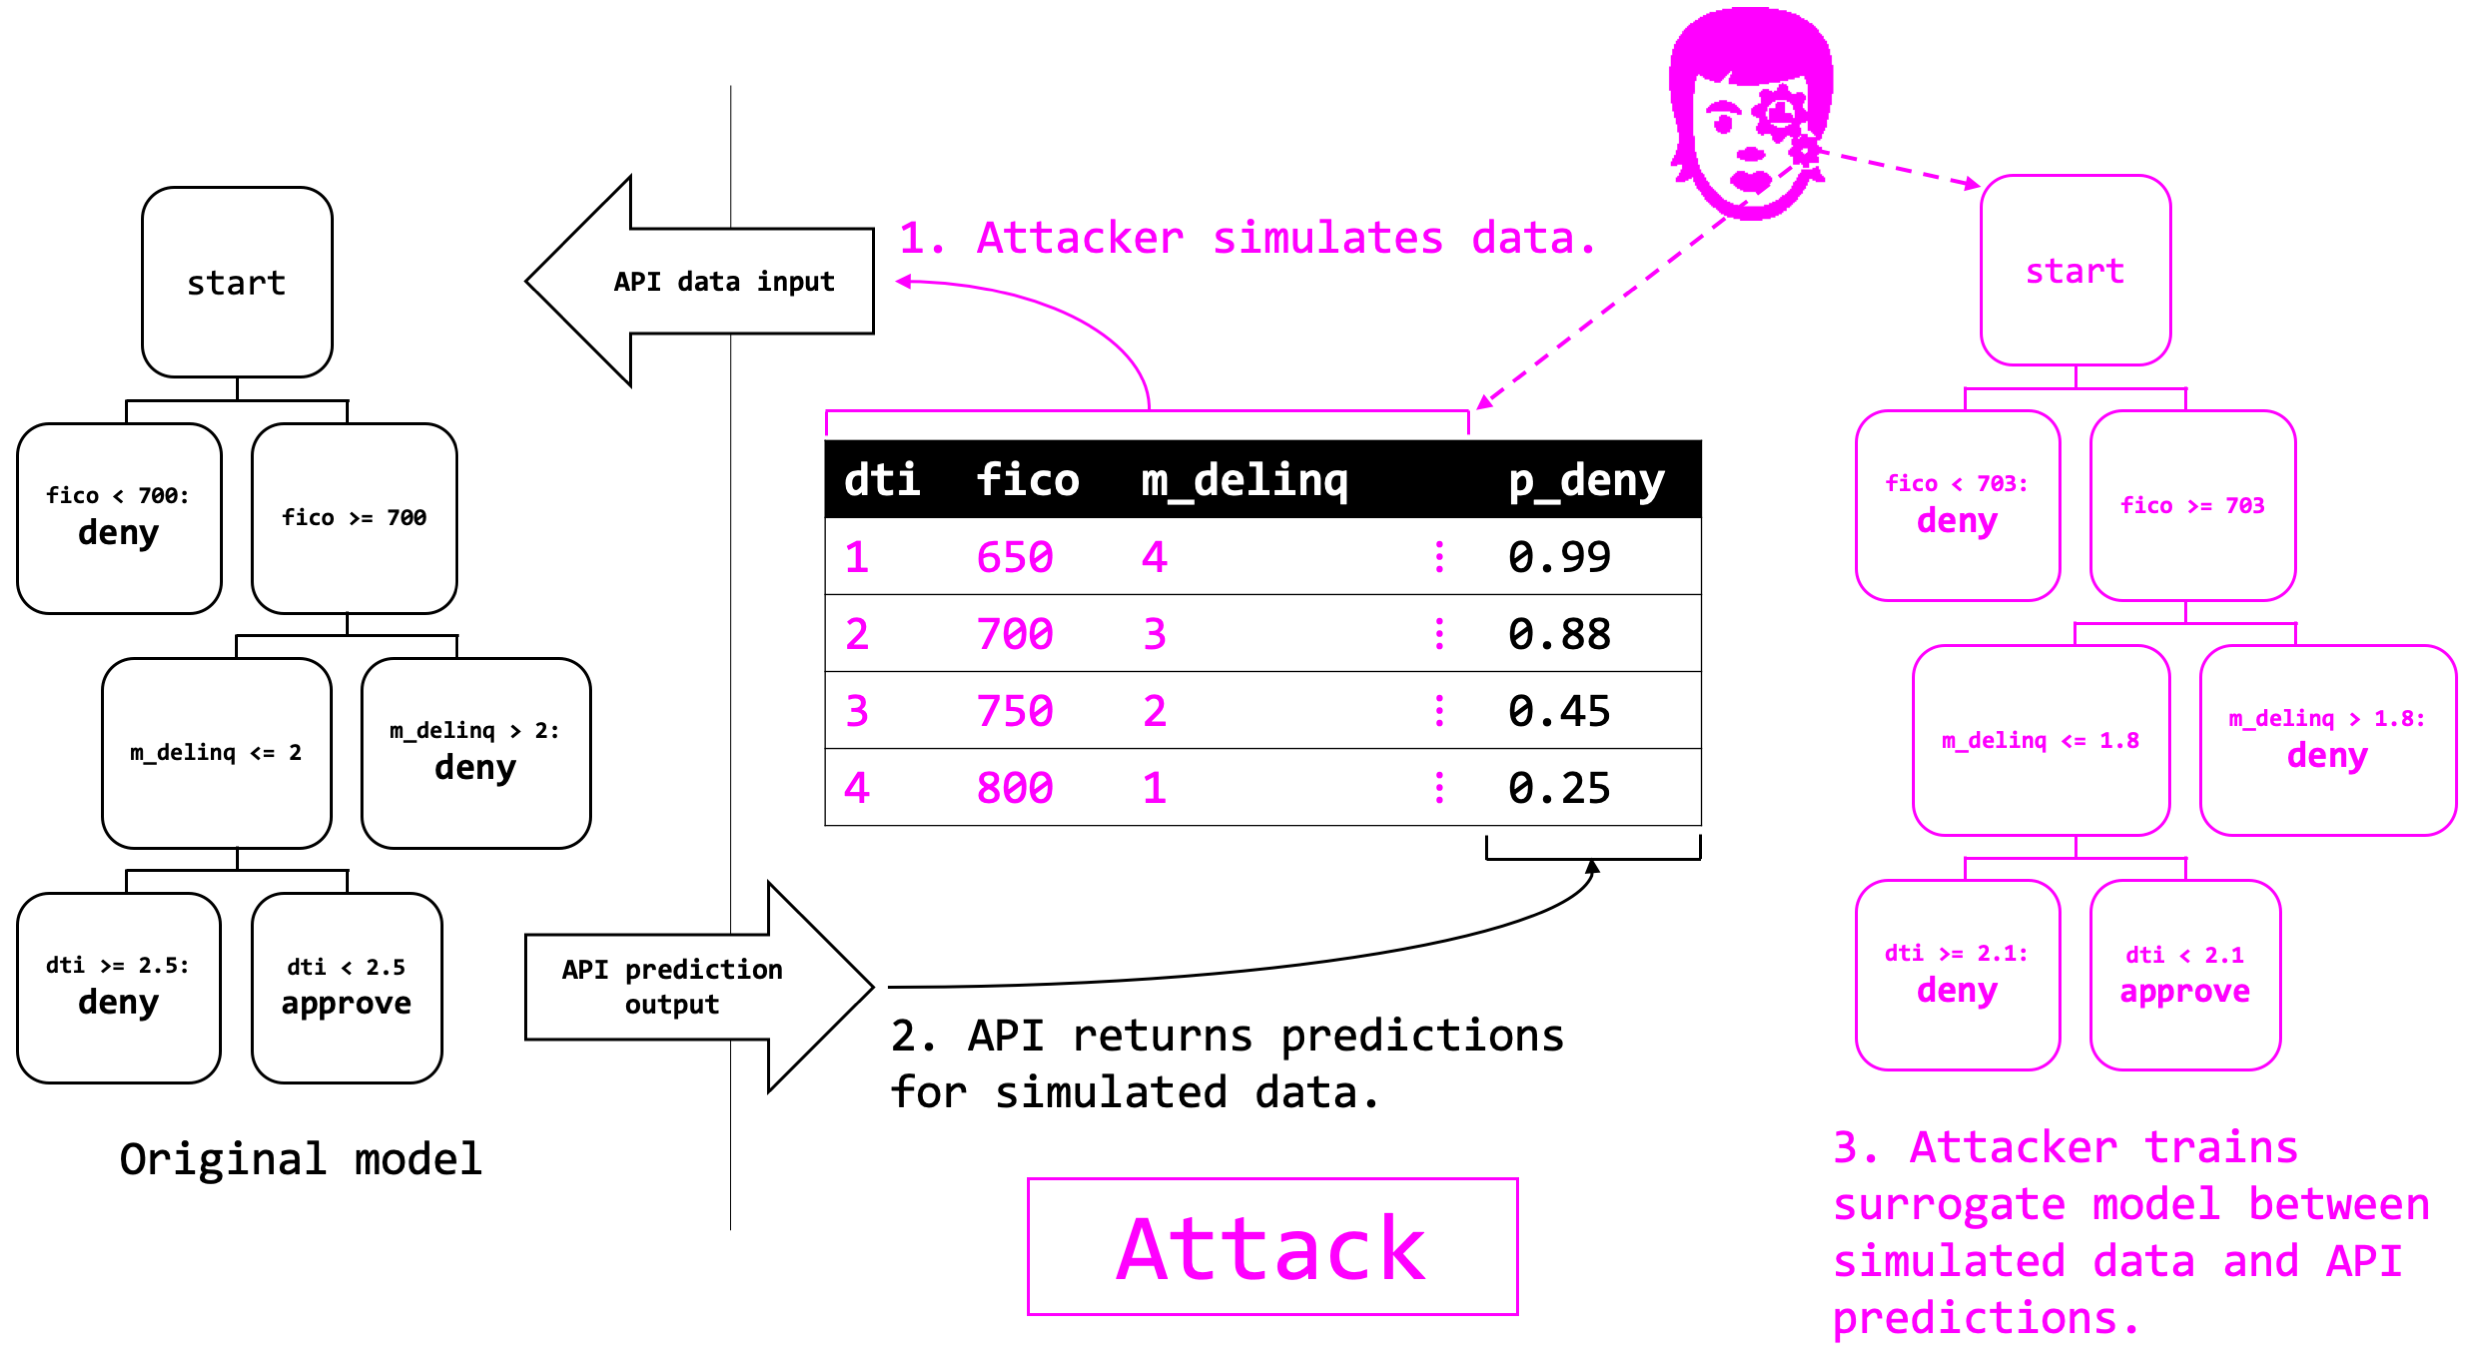
\includegraphics[height=150pt]{img/inversion.PNG}
					\end{center}
				\end{figure}	

			\end{frame}
		
			\begin{frame}[label={slide:inversion_defense}]
		
				\frametitle{Surrogate Model Inversion Attacks: \textbf{Defenses}}
				\begin{itemize}
					\item \textbf{Authentication}: Always authenticate users of your model’s API or other endpoints.
					\item \textbf{Defensive watermarks}: Add subtle or unusual information to your model’s predictions to aid in forensic analysis if your model is hacked or stolen.
					\item \textbf{Throttling}: Consider artificially slowing down your prediction response times, especially after anomalous behavior is detected.
					\item \textbf{White-hat surrogate models}: Try to build your own surrogate models as a white-hat hacking exercise to see what an attacker could learn about your public models.
				\end{itemize}
				
			\end{frame}
		

%-------------------------------------------------------------------------------
		\subsection{Membership Inference}
%-------------------------------------------------------------------------------

			\begin{frame}
		
				\frametitle{Membership Inference Attacks: \textbf{What?}}		
				\small Due to lax security or a distributed attack on your model API or other model endpoint ... 
			
				\begin{itemize}
					\item this two-stage attack begins with a surrogate model inversion attack (see Slide: \ref{slide:inversion}).
					\item A second-level surrogate is then trained to discriminate between rows of data in, and not in, the first-level surrogate's training data.
					\item The second-level surrogate can dependably reveal whether a row of data was in, or not in, your training data \cite{membership_inference}.
				\end{itemize}
				
Simply knowing if a person was in, or not in, a training dataset can be a violation of individual or group privacy. However, when carried out to the fullest extent, a membership inference attack can allow a bad actor to \textbf{rebuild your sensitive training data}!\normalsize	

			\end{frame}
	
			\begin{frame}[label={slide:membership}]
		
				\frametitle{Membership Inference Attacks: \textbf{How?}}		
			
				\begin{figure}[htb]
					\begin{center}
						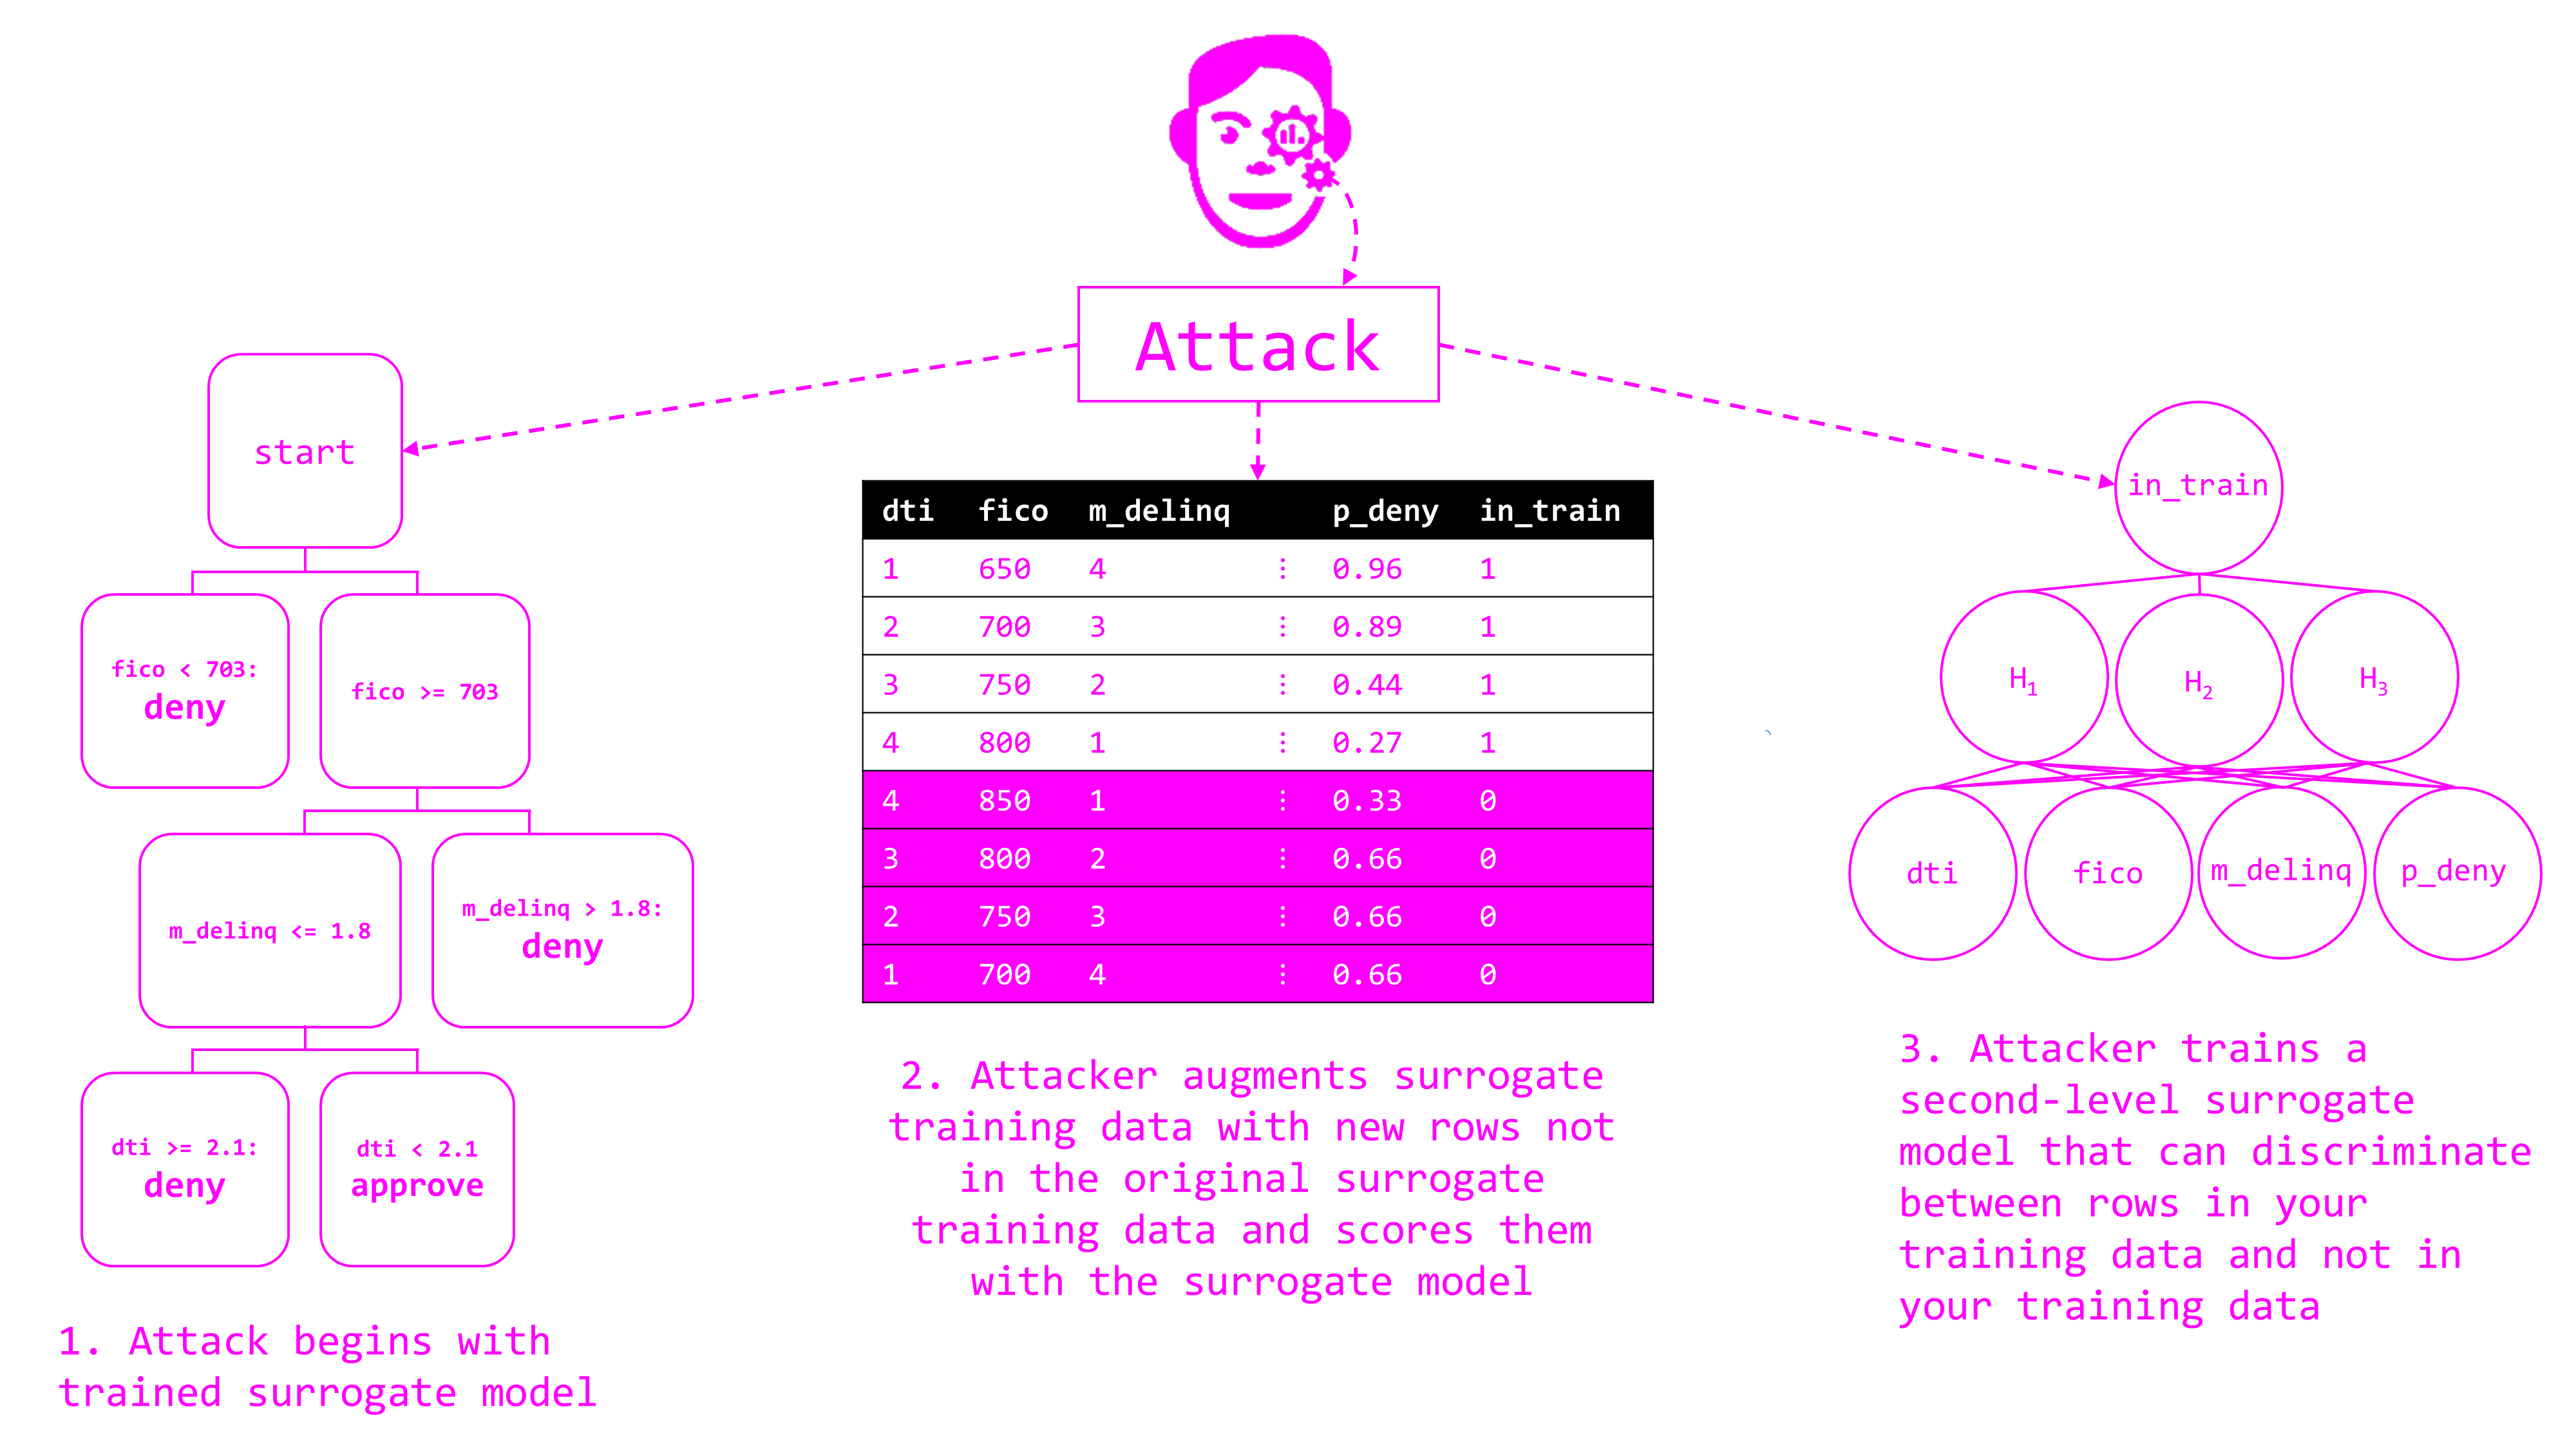
\includegraphics[height=150pt]{img/membership.PNG}
					\end{center}
				\end{figure}	

			\end{frame}
			
			\begin{frame}
		
				\frametitle{Membership Inference Attacks: \textbf{Defenses}}		
			
				\begin{itemize}
					\item See Slide \ref{slide:inversion_defense}.
				\item \textbf{Monitor for training data}: Monitor your production scoring queue for data that closely resembles any individual used to train your model. Real-time scoring of rows that are extremely similar or identical to data used in training, validation, or testing should be recorded and investigated.
				\end{itemize}

			\end{frame}
	
%-------------------------------------------------------------------------------
		\subsection{Adversarial Examples}
%-------------------------------------------------------------------------------
	
			\begin{frame}
		
				\frametitle{Adversarial Example Attacks: \textbf{What?}}		

Due to lax security or a distributed attack on your model API or other model endpoint, hackers or competitors simulate data, submit it, receive predictions, and learn by systematic trial-and-error ... 		
				\begin{itemize}
					\item your proprietary business logic.
					\item how to game your model to dependably receive a desired outcome. 
				\end{itemize}
				\vspace{10pt}
Adversarial example attacks can also be enhanced, tested, and hardened using models trained from surrogate model inversion attacks (see Slide \ref{slide:inversion}).

			\end{frame}	
	
			\begin{frame}[label={slide:adversary}]
		
				\frametitle{Adversarial Example Attacks: \textbf{How?}}		
			
				\begin{figure}[htb]
					\begin{center}
						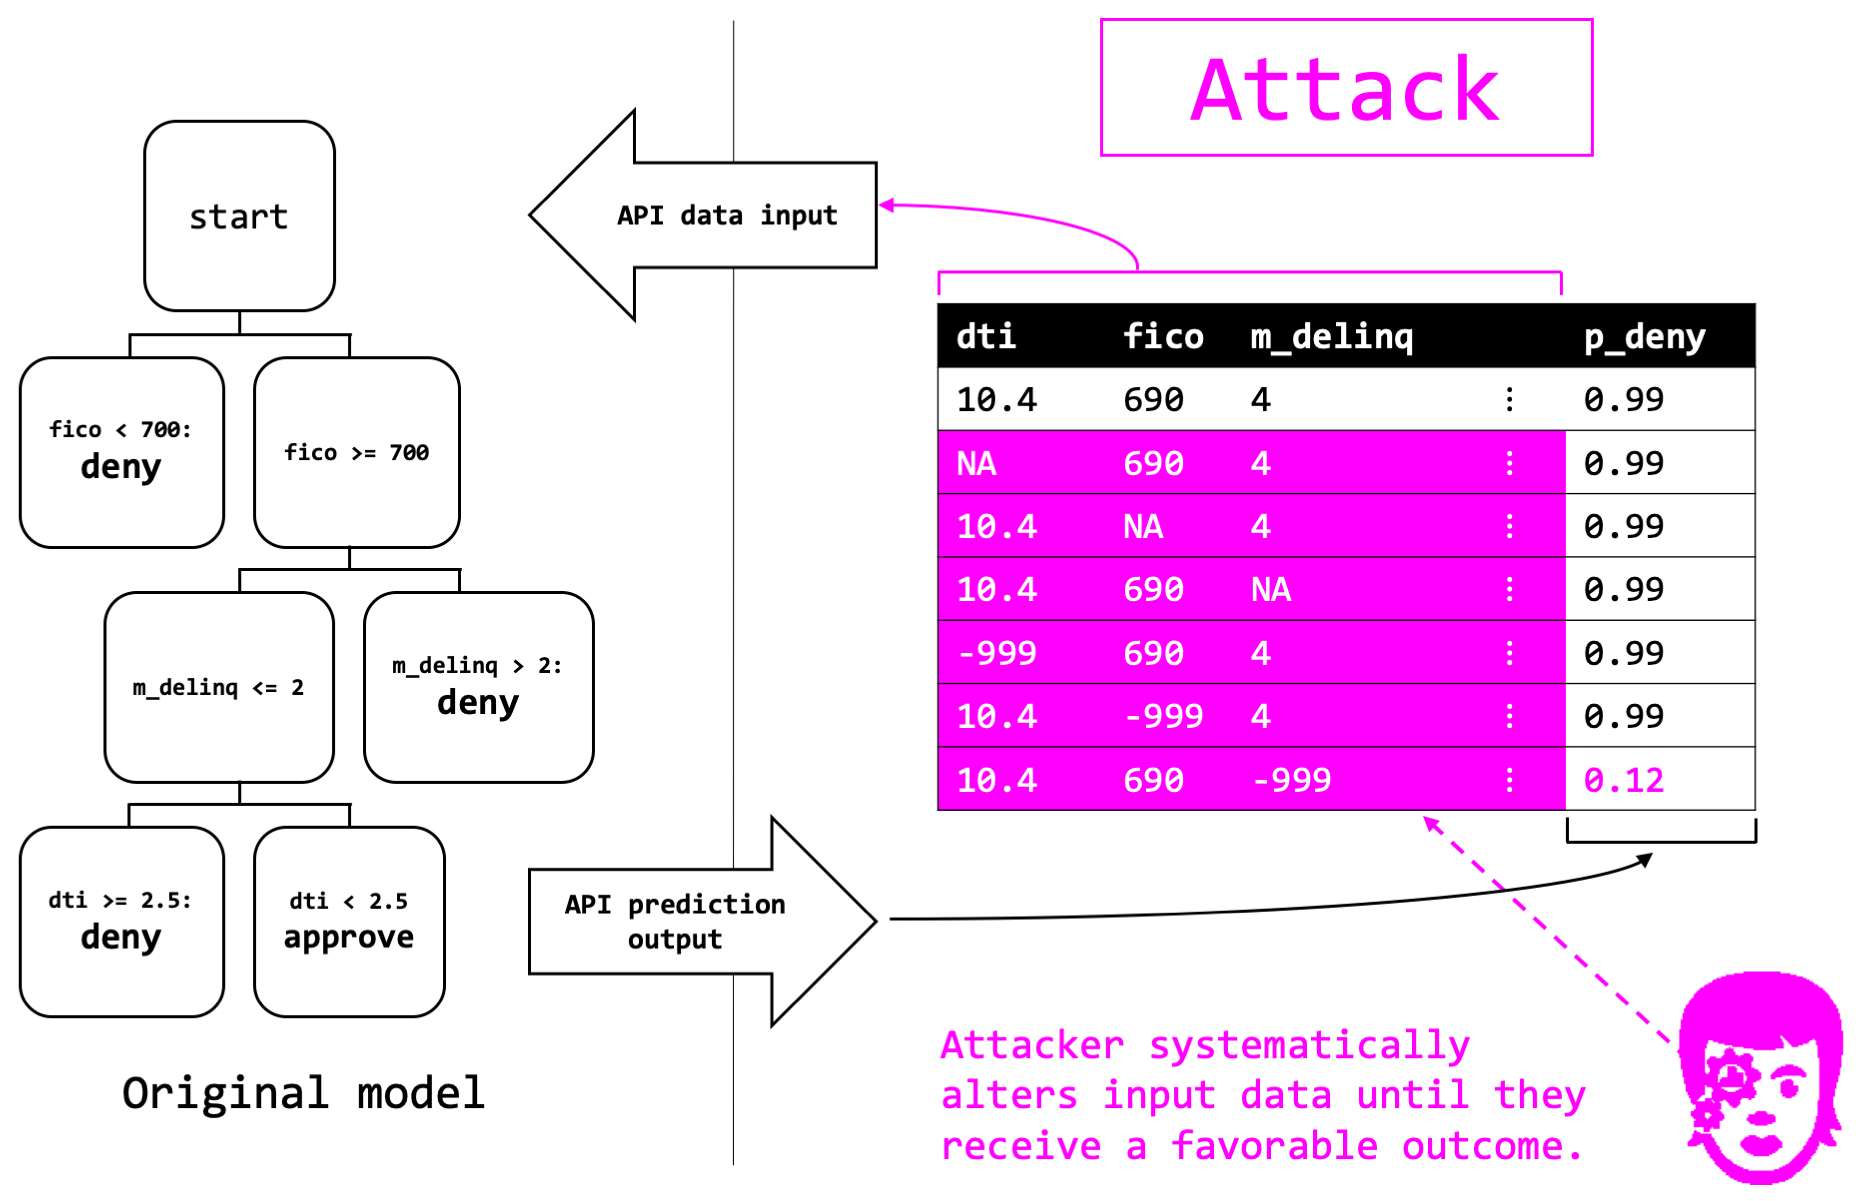
\includegraphics[height=150pt]{img/adversary.PNG}
					\end{center}
				\end{figure}	

			\end{frame}	
			
			\begin{frame}
		
				\frametitle{Adversarial Example Attacks: \textbf{Defenses}}		
			
				\begin{itemize}
					\item \textbf{Anomaly detection}: See Slide \ref{slide:watermark_defense}. 
					\item \textbf{Authentication}: See Slide \ref{slide:inversion_defense}. 
					\item \textbf{Benchmark models}: Always compare complex model predictions to trusted linear model predictions. If the two model’s predictions diverge beyond some acceptable threshold, review the prediction before you issue it.
					\item \textbf{Throttling}: See Slide \ref{slide:inversion_defense}. 
					\item \textbf{Model monitoring}: Watch your model in real-time for strange prediction behavior.
					\item \textbf{White-hat sensitivity analysis}: Try to trick your own model by seeing its outcome on many different combinations of input data values.
					\item \textbf{White-hat surrogate models}: See Slide \ref{slide:inversion_defense}. 
				\end{itemize}

			\end{frame}

%-------------------------------------------------------------------------------
		\subsection{Impersonation}
%-------------------------------------------------------------------------------

			\begin{frame}
		
				\frametitle{Impersonation Attacks: \textbf{What?}}		
Bad actors learn ... 
				\begin{itemize}
					\item by inversion or adversarial example attacks (see Slides \ref{slide:inversion}, \ref{slide:adversary}), the attributes favored by your model and then impersonate them.
					\item by disparate impact analysis (see Slide \ref{slide:data_poisoning_defense}), that your model is discriminatory (e.g. \href{https://www.propublica.org/article/machine-bias-risk-assessments-in-criminal-sentencing}{Propublica and COMPAS}, \href{https://medium.com/@Joy.Buolamwini/response-racial-and-gender-bias-in-amazon-rekognition-commercial-ai-system-for-analyzing-faces-a289222eeced}{Gendershades and Rekognition}), and impersonate your model's privileged class to receive a favorable outcome.\footnote{This presentation makes no claim on the quality of the analysis in Angwin et al. (2016), which has been criticized, but is simply stating that such cracking is possible \cite{angwin16,}, \cite{flores2016false}.}
				\end{itemize}
				
			\end{frame}

			\begin{frame}
		
				\frametitle{Impersonation Attacks: \textbf{How?}}		
			
				\begin{figure}[htb]
					\begin{center}
						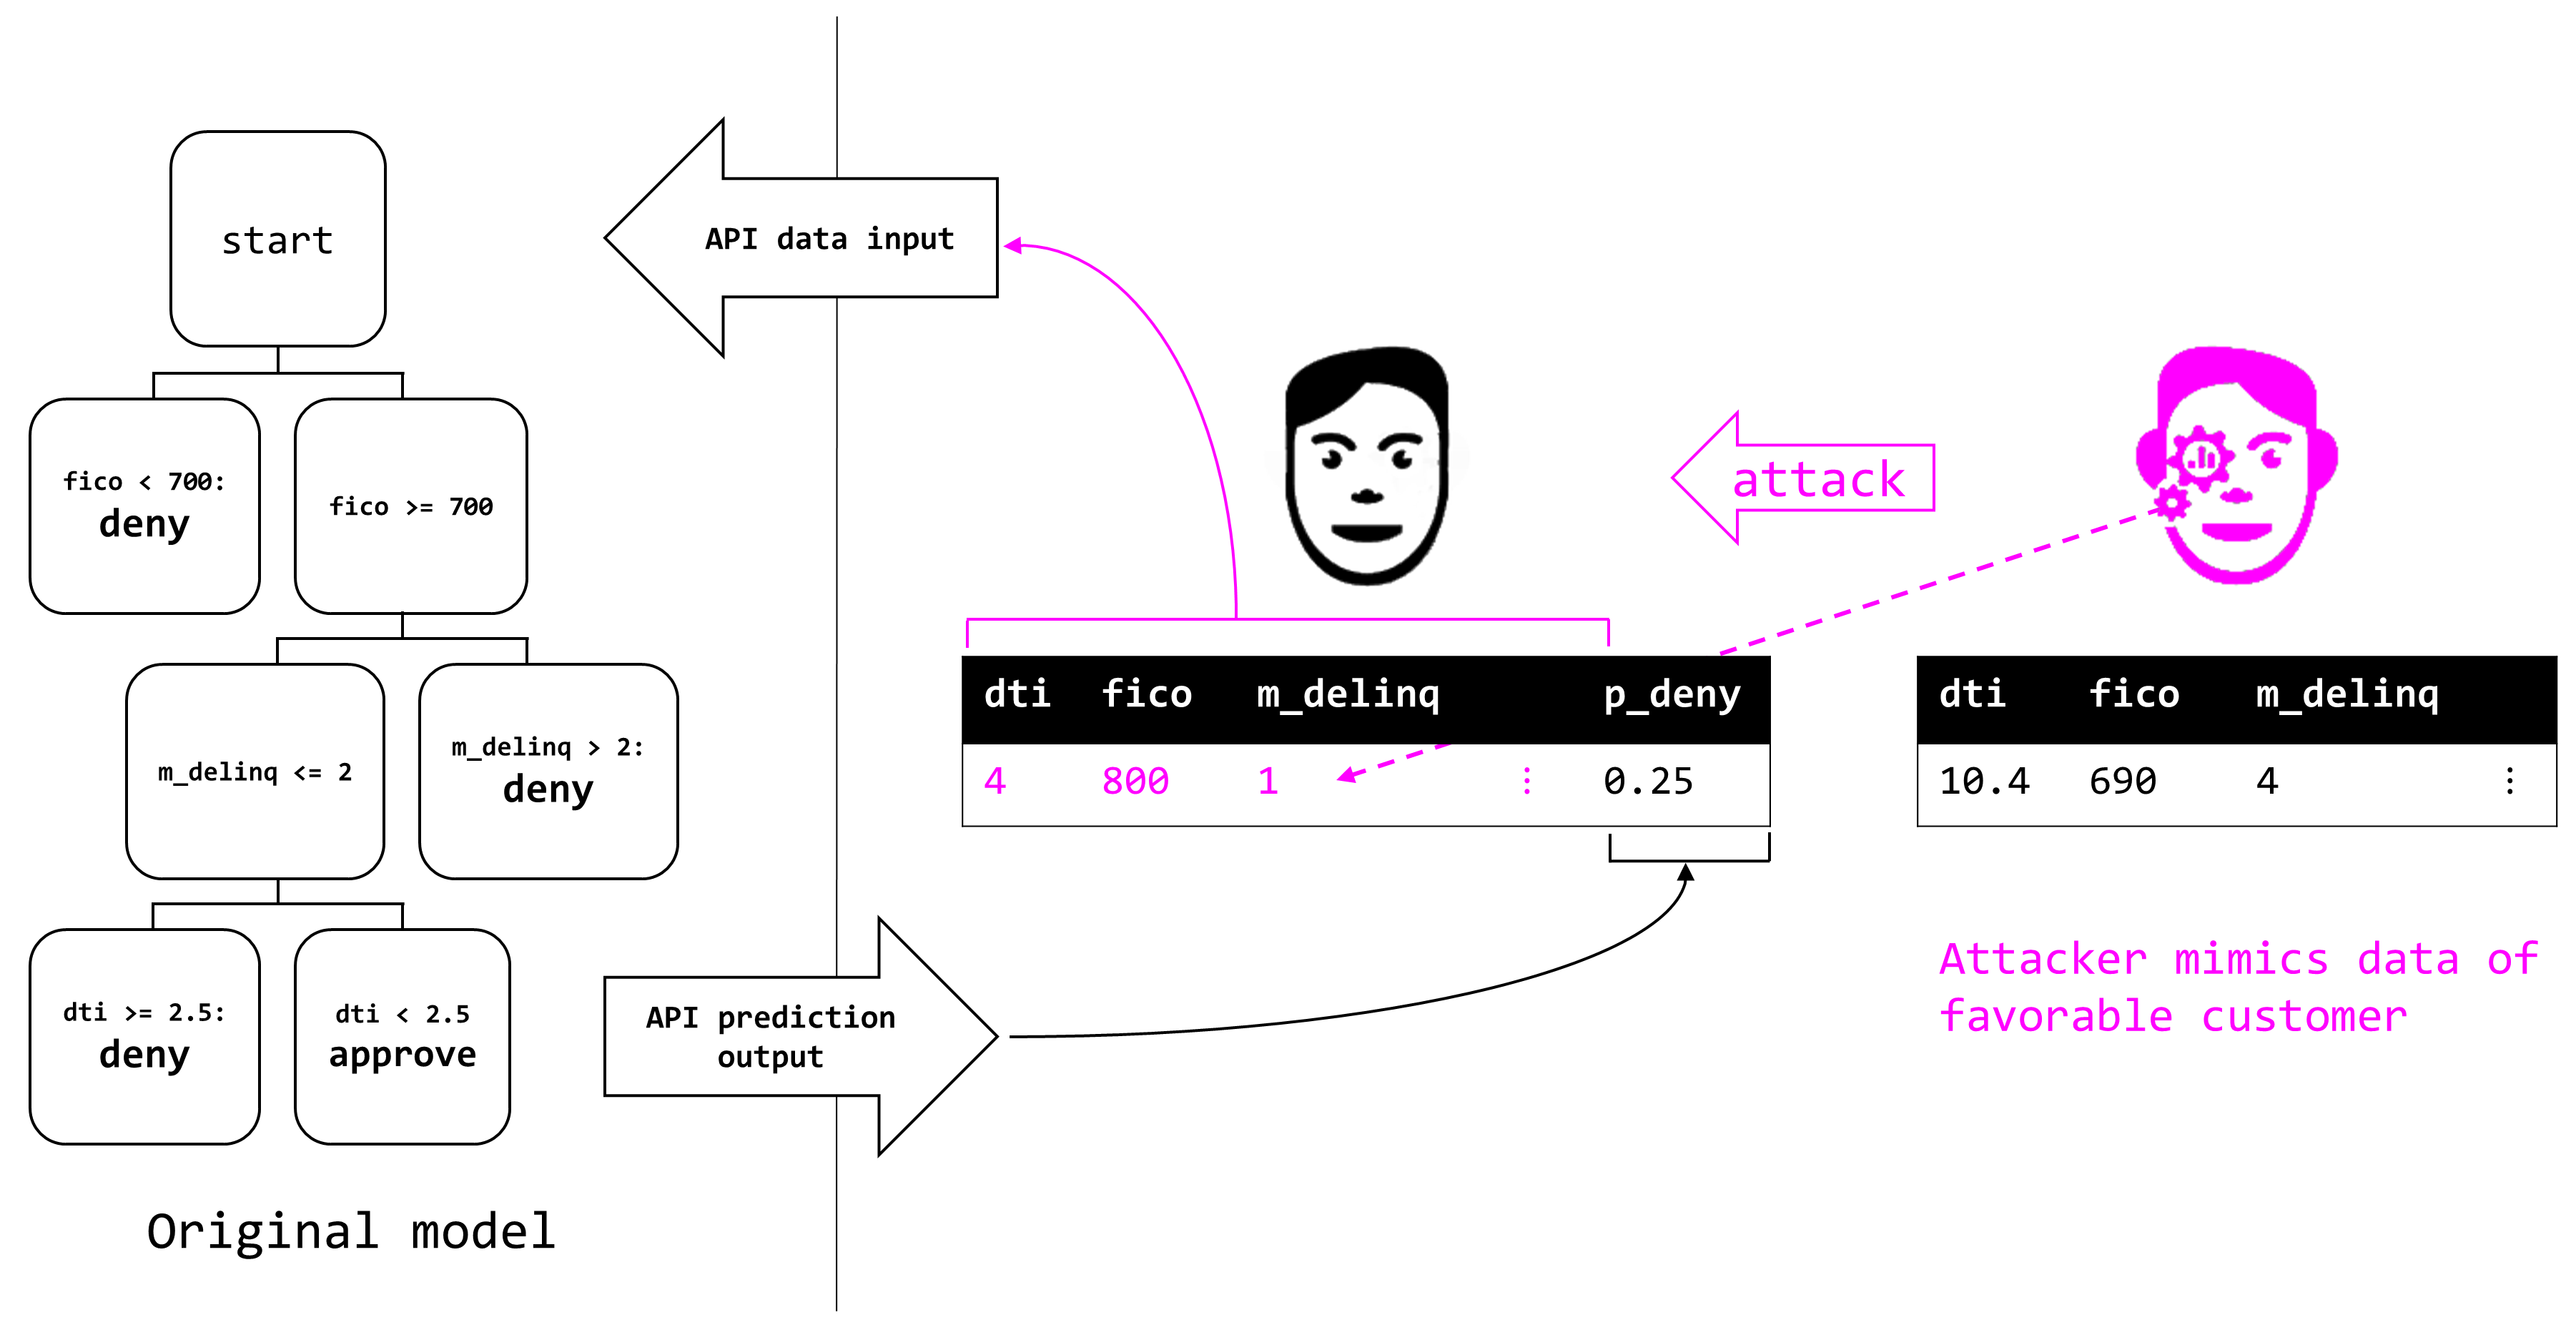
\includegraphics[height=150pt]{img/imperson.PNG}
					\end{center}
				\end{figure}	
				
			\end{frame}
			
			\begin{frame}
		
				\frametitle{Impersonation Attacks: \textbf{Defenses}}		
			
				\begin{itemize}
					\item \textbf{Authentication}: See Slide \ref{slide:inversion_defense}. 
					\item \textbf{Disparate impact analysis}: See Slide \ref{slide:data_poisoning_defense}.
					\item \textbf{Model monitoring}: Watch for too many similar predictions in real-time. Watch for too many similar input rows in real-time.
				\end{itemize}
				
			\end{frame}

%-------------------------------------------------------------------------------
	\section{General Concerns}
%-------------------------------------------------------------------------------

			\begin{frame}[t, allowframebreaks]	
		
				\frametitle{General concerns}	
				\small 
				\begin{itemize}
					\item \textbf{Black-box models}: Over time a motivated, malicious actor could learn more about your own black-box model than you know and use this knowledge imbalance to attack your model \cite{papernot2018marauder}.
					\item \textbf{Black-hat eXplainable AI (XAI)}:  While XAI can enable human learning from machine learning, regulatory compliance, and appeal of automated decisions, it can also make ML hacks easier and more damaging \cite{shokri2019privacy}.
					\item \textbf{Distributed-denial-of-service (DDOS) attacks}: Like any other public-facing service, your model could be attacked with a DDOS attack that has nothing to do with machine learning.
					\item \textbf{Distributed systems and models}: Data and code spread over many machines provides a larger, more complex attack surface for a malicious actor.
					\item \textbf{Package dependencies}: Any package your modeling pipeline is dependent on could potentially be hacked to conceal an attack payload.
				\end{itemize}
				\normalsize

			\end{frame}

%-------------------------------------------------------------------------------
	\section{General Solutions}
%-------------------------------------------------------------------------------
	
%-------------------------------------------------------------------------------
		\subsection{General Solutions}
%-------------------------------------------------------------------------------
	
			\begin{frame}[t, allowframebreaks]	
		
				\frametitle{General Solutions}	
				\small
				\begin{itemize}
					\item \textbf{Authenticated access and prediction throttling}: for prediction APIs and other model endpoints.
					\item \textbf{Benchmark models}: Always compare complex model predictions to less complex (and hopefully less hackable) model predictions. For traditional, low signal-to-noise data mining problems, predictions should probably not be too different. If they are, investigate them.
					\item \textbf{Encrypted, differentially private, or federated training data}: Properly implemented, encrypted, differentially private, or federated training data can thwart many types of attacks. (Improperly implemented, these technologies simply create a broader attack surface or hinder forensic efforts.)		
					\item \textbf{Interpretable, fair, or private models}: Some types of nonlinear models are designed to be directly interpretable, less discriminatory, or harder to hack. Consider using them. In addition to models like LFR and PATE, also checkout \href{https://github.com/h2oai/h2o-3/blob/master/h2o-py/demos/H2O_tutorial_gbm_monotonicity.ipynb}{monotonic GBMs} and \href{https://christophm.github.io/interpretable-ml-book/rulefit.html}{Rulefit}.
					\item \textbf{Model documentation, management, and monitoring}: Take an inventory of your predictive models. All production models should be documented well-enough that a new employee could diagnose whether its current behavior is notably different from its intended or original behavior. Also keep details about who trained what model and on what data. Additionally, analyze the inputs and predictions of deployed models on live data. If they seem strange, investigate the problem.	
					\item \textbf{Model debugging and testing, and white-hat hacking}: Test your models for accuracy, fairness, and privacy before deploying them. Train white-hat surrogate models and apply XAI techniques to them to see what a hackers can see. 
					\item \textbf{System monitoring and profiling}: Train an autoencoder–based anomaly detection metamodel on your entire predictive modeling system’s operating statistics—the number of predictions in some time period, latency, CPU, memory and disk loads, the number of concurrent users, and everything else you can get your hands on—and then closely monitor this metamodel for anomalies.
				\end{itemize}
				\normalsize

			\end{frame}

%-------------------------------------------------------------------------------
		\subsection{Low-Risk ML Blueprint}
%-------------------------------------------------------------------------------

		\begin{frame}
		
			\frametitle{A Blueprint for Low-Risk Machine Learning \footnote{See: \url{ https://github.com/jphall663/hc_ml} for more information.} }		
			
			\begin{figure}[htb]
				\begin{center}
					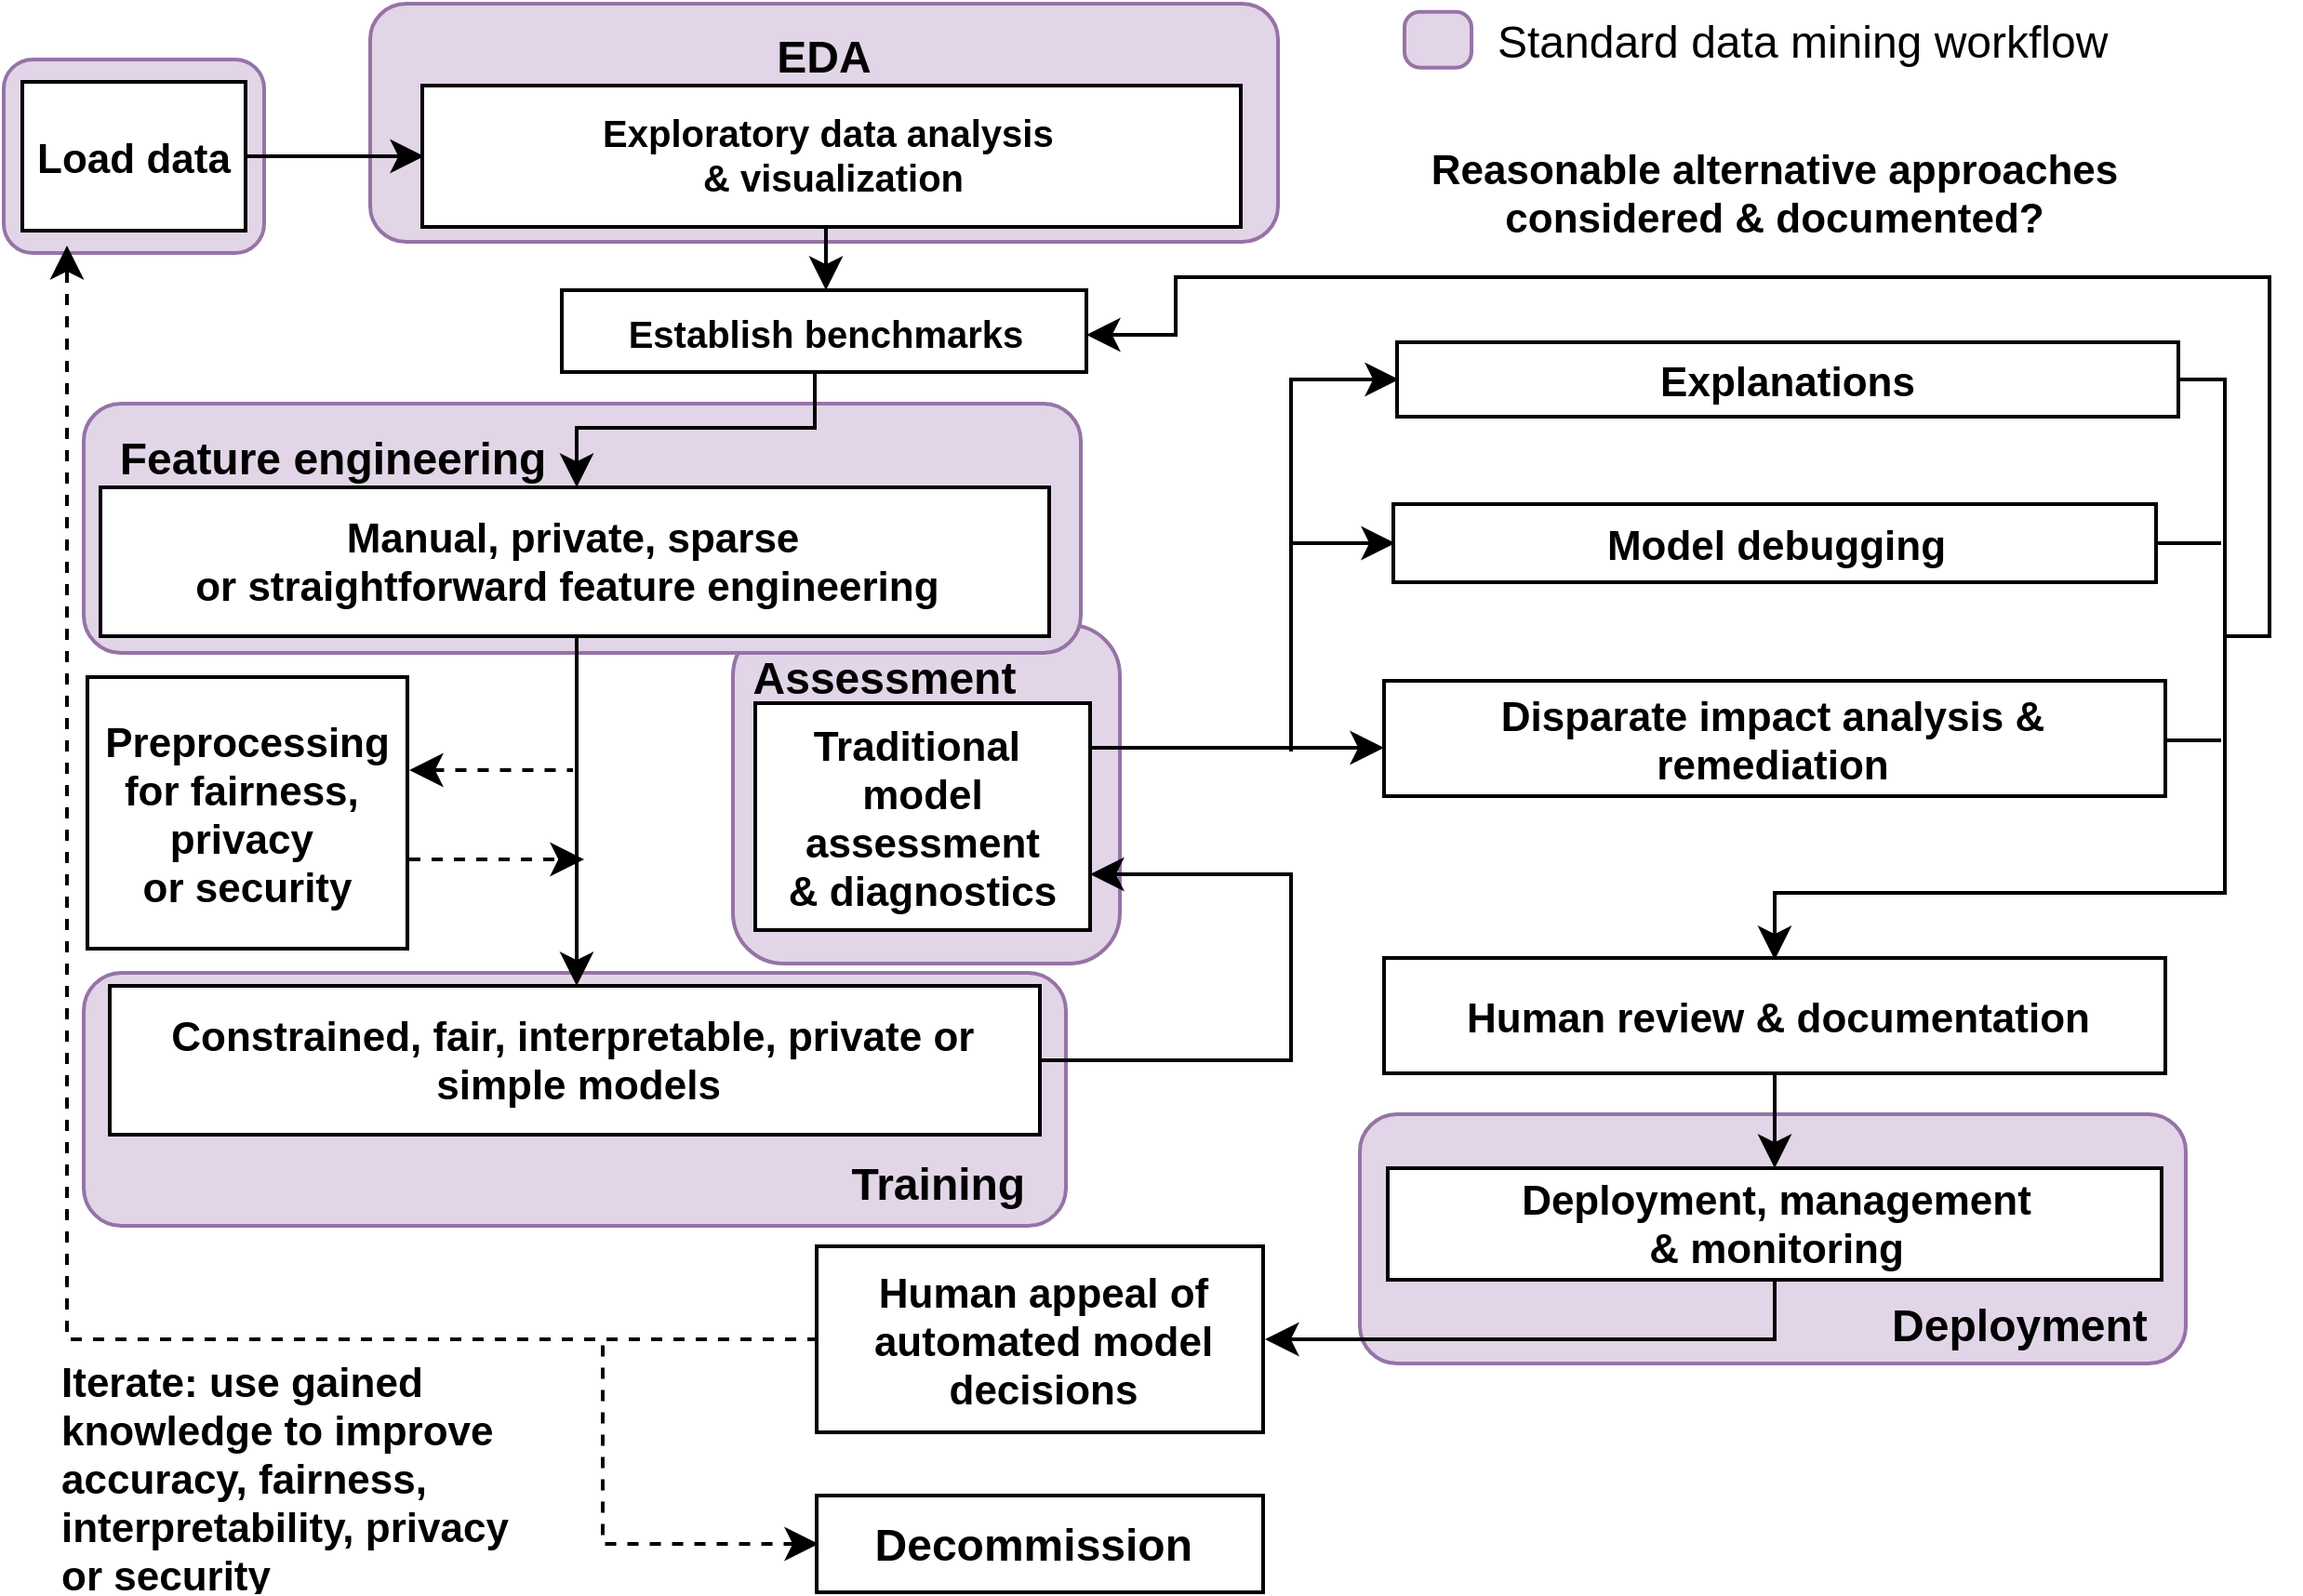
\includegraphics[height=140pt]{img/blueprint.png}
				\end{center}
			\end{figure}	

		\end{frame}

%-------------------------------------------------------------------------------
	\section{Summary}
%-------------------------------------------------------------------------------

		\begin{frame}
		
			\frametitle{Summary}		
			
			\begin{itemize}
				\item ML hacking is still probably rare and exotic, but new XAI techniques can make nearly all ML attacks easier and more damaging.
				\item Beware of insider threats, especially organized extortion of insiders. 
				\item Open, public prediction APIs are a privacy and security nightmare. 
				\item Your competitors could be gaming or stealing your public predictive models. Do your end user license agreements (EULA) or terms of service (TOS) explicitly prohibit this?
				\item Best practices around IT security, model management, and model monitoring are good defenses.
			\end{itemize}
		
		\end{frame}


%-------------------------------------------------------------------------------
%	References
%-------------------------------------------------------------------------------

	\begin{frame}[t, allowframebreaks]
	
		\frametitle{References}	
		
			This presentation:\\
			\footnotesize{\url{https://github.com/jphall663/secure_ML_ideas}}\normalsize
			
			\vspace{10pt}
		
			\textit{Proposals for Model Vulnerability and Security}:\\
			\footnotesize{\url{https://www.oreilly.com/ideas/proposals-for-model-vulnerability-and-security}}\normalsize
			
			\vspace{10pt}
			
			\textit{Can Your Machine Learning Model Be Hacked?!'}:\\
			\footnotesize{\url{https://www.h2o.ai/blog/can-your-machine-learning-model-be-hacked/}}
			
		
		\framebreak		
		
		\printbibliography
		
	\end{frame}

\end{document}